\section{NaFSI solutions in EMIM-FSI ionic liquid}
\label{section:emim-fsi}

This section presents results for the solutions of NaFSI salt in the EMIM-FSI ionic liquid at different concentrations. Such electrolytes were experimentally investigated in~\cite{na-fsi,na-il-1}. This part is an extension to studies which were the basis for the Master of Science thesis of the author of this work~\cite{msc-thesis}. Most of the results described here were published in the~paper~\cite{emim-fsi}.

\begin{table}[ht]
    \centering
    \caption{Compositions of (NaFSI)$_{x}$(EMIM-FSI)$_{1-x}$ systems}
    \label{tab:emim-fsi-compositions}
    \begin{tabular}{cccc}
      \toprule
      \multicolumn{4}{c}{classical MD} \\
      x & Na$^{+}$ & EMIM$^{+}$ & FSI$^{-}$ \\
      \midrule
      0 & 0 & 175 & 175 \\
      0.1 & 19 & 171 & 190 \\
      0.2 & 40 & 160 & 200 \\
      0.3 & 66 & 154 & 220 \\
      0.4 & 94 & 141 & 235 \\
      0.5 & 129 & 129 & 258 \\
      \midrule
      \multicolumn{4}{c}{ab initio MD} \\
      x & Na$^{+}$ & EMIM$^{+}$ & FSI$^{-}$ \\
      \midrule
      0 & 0 & 18 & 18 \\
      0.2 & 4 & 16 & 20 \\
      0.5 & 13 & 13 & 26 \\
      \bottomrule
    \end{tabular}    
\end{table}

\subsection{System details}
\label{subsection:emim-fsi-na-fsi-system-details}

MP2 method was used for the geometry optimizations of different conformers of FSI$^{-}$ anion and Na$^{+}$FSI$^{-}$ pairs in vacuum.

The compositions of the systems simulated in MD are presented in Table~\ref{tab:emim-fsi-compositions}.

For classical MD pressure $p = 1$~atm and temperature $T = 298$~K were used. After 100-150~ns of equilibration trajectories for all systems were recorded for 1~$\mu$s in simulations using DP-FF and NP-FF with a~time step of 1.0~fs.

AIMD was performed for selected concentrations of sodium salt. Initial structures were chosen from equilibrated NVT simulations in classical polarizable FF. Two systems with $x = 0$ and $x = 0.2$ were simulated, and three with $x = 0.5$. The temperature was set to 298~K. Time step equal 1.0~fs was used and 30~ps of the trajectory was recorded for each system.

\subsection{Results}

\begin{figure}[ht]
    \centering
    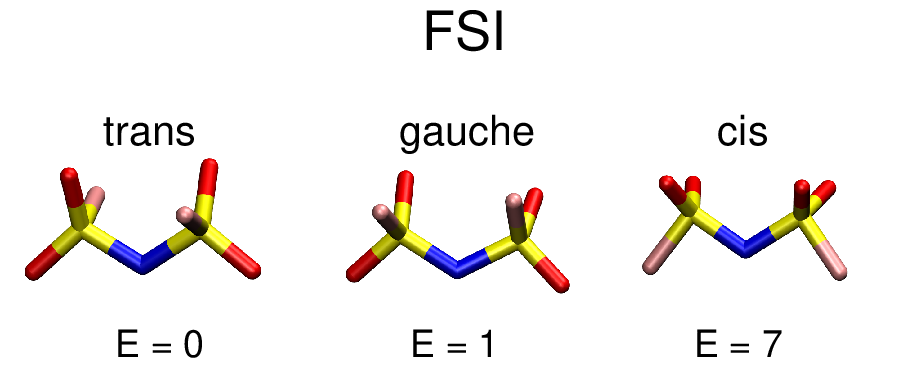
\includegraphics[width=0.4\textwidth]{img/3-structural-data-from-md-simulations/1-emim-fsi/conformers/fsi-conformers.png}
    \caption{Conformers of the FSI$^{-}$ anion with their relative energies in kcal/mol}
    \label{fig:emim-fsi-fsi-conformers}
\end{figure}

\begin{figure}[ht]
    \centering
    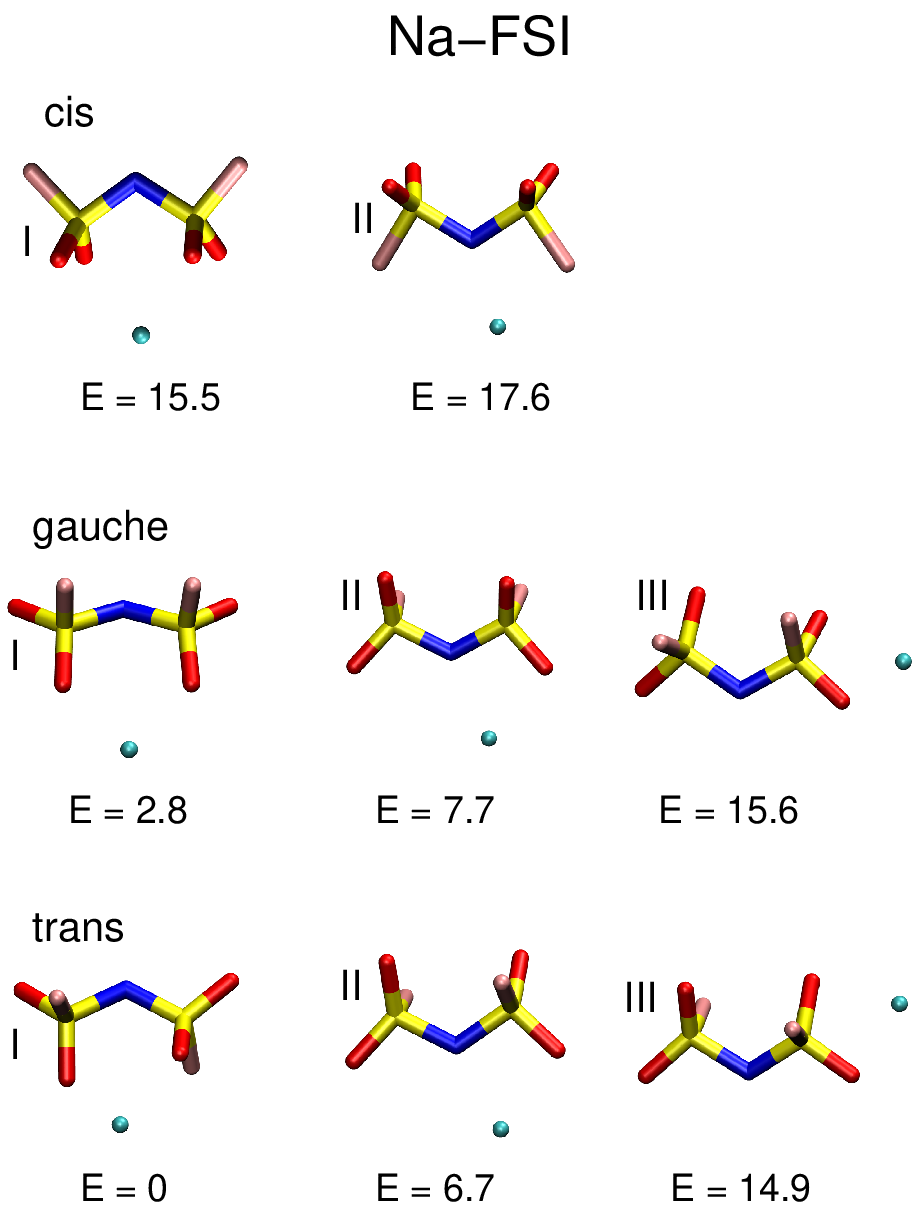
\includegraphics[width=0.4\textwidth]{img/3-structural-data-from-md-simulations/1-emim-fsi/conformers/na-fsi-conformers.png}
    \caption{Conformers of the Na-FSI pairs with their relative energies in kcal/mol}
    \label{fig:emim-fsi-na-fsi-conformers}
\end{figure}

Three conformers of the FSI$^{-}$ anion: cis, gauche and trans were optimized at the MP2 level of theory, their structures with relative energies in kcal/mol are presented in Figure~\ref{fig:emim-fsi-fsi-conformers}. It is visible that the lowest energy is obtained for the trans conformer and is followed by gauche. The energy difference between the cis and trans or gauche conformers is rather big and suggests that appearance of cis structure in the liquid is unlikely. The lowest energy for the trans structure stands in an agreement with experimental results obtained from Raman spectroscopy~\cite{raman-interactions-2}.

\begin{figure}[ht]
    \centering
    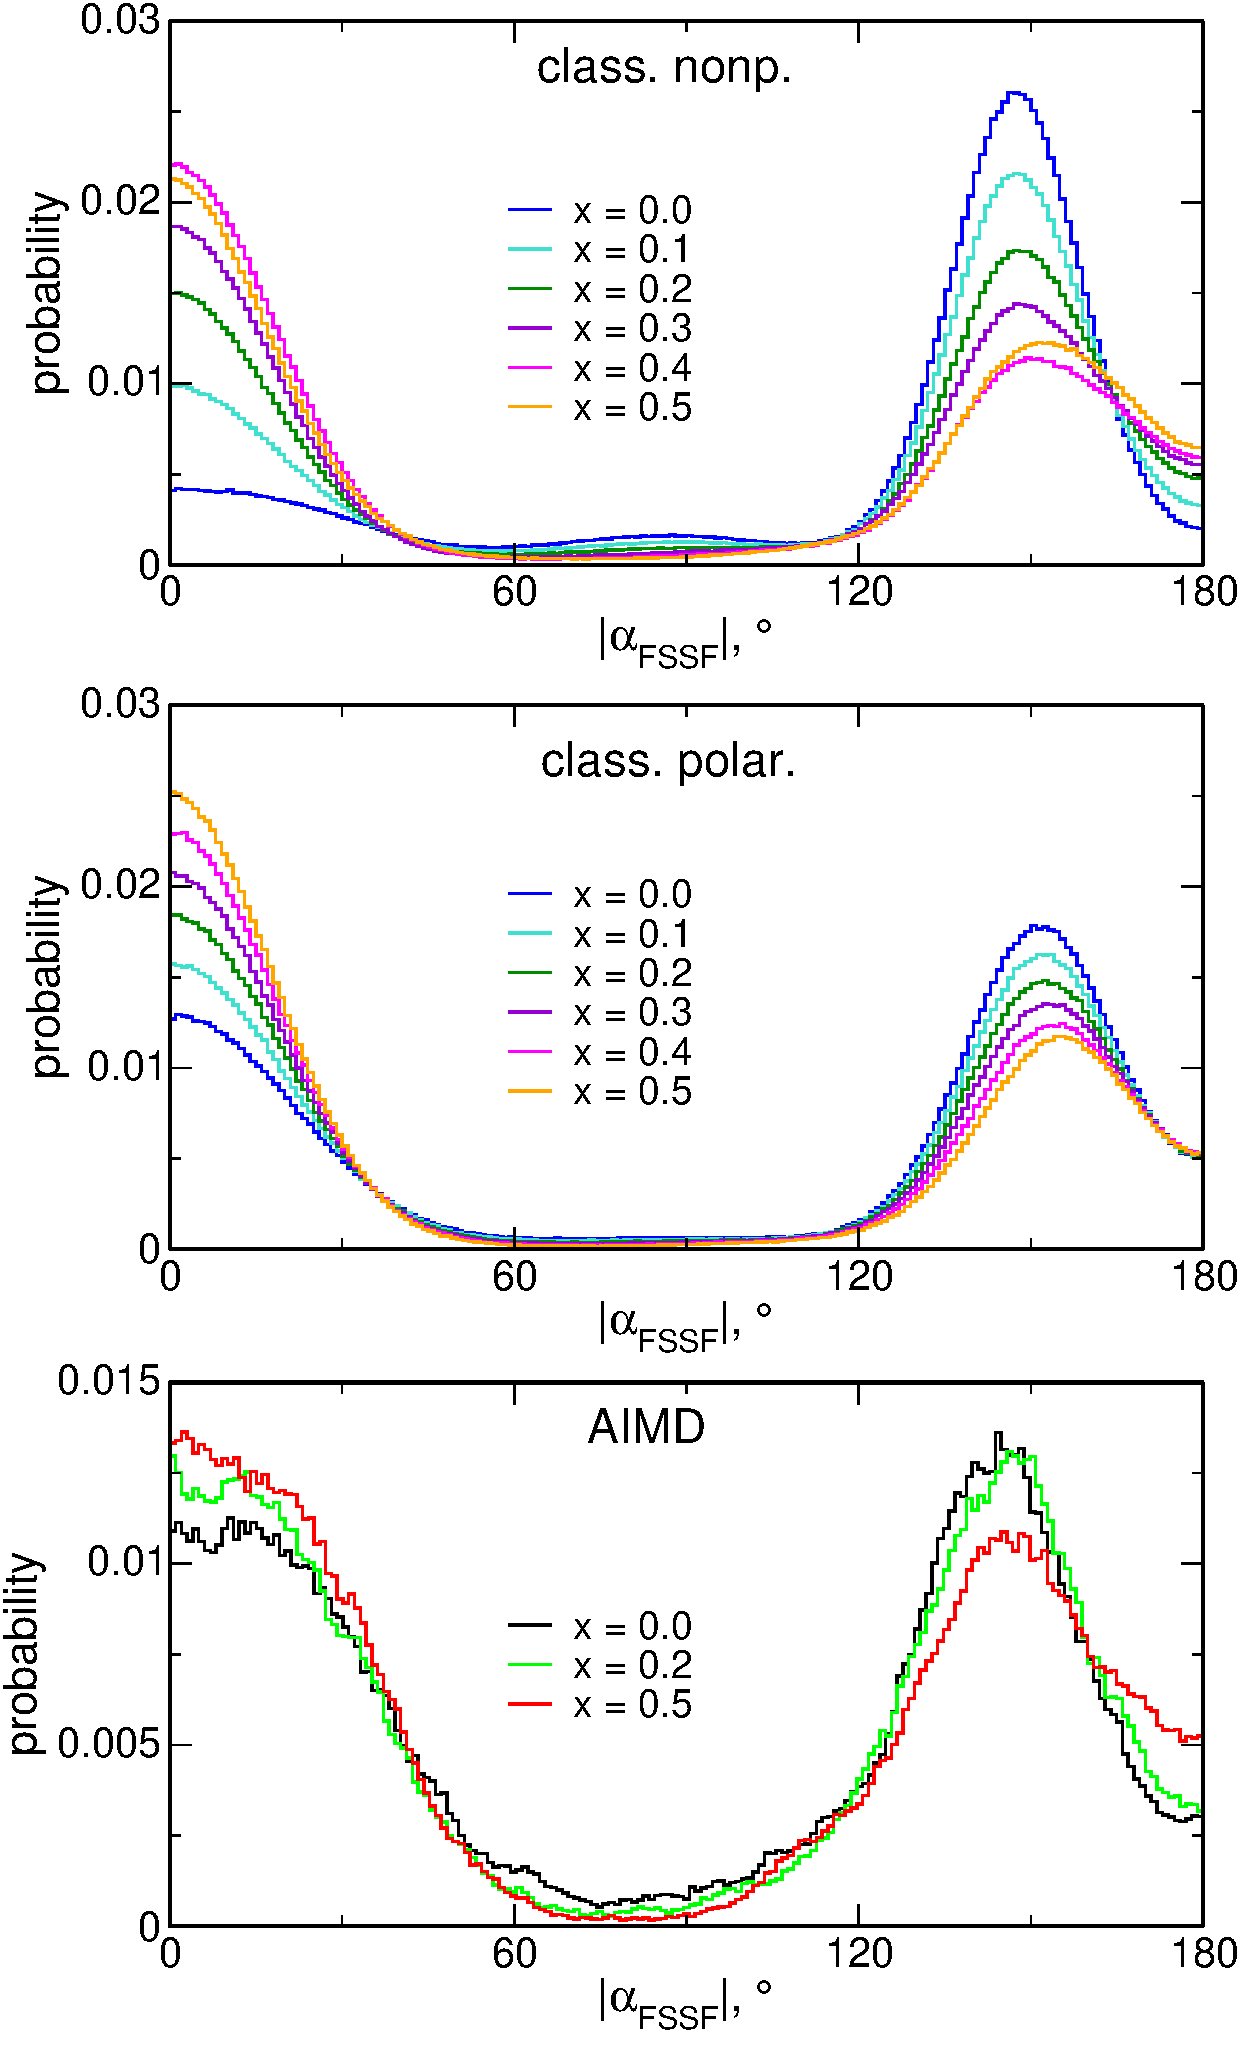
\includegraphics[width=0.45\textwidth]{img/3-structural-data-from-md-simulations/1-emim-fsi/conformers/angle-distribution.png}
    \caption{Histograms of the FSSF angle in simulated systems for classical and ab initio MD}
    \label{fig:emim-fsi-angle-distribution}
\end{figure}

Analogical analysis was performed for ion pairs Na$^{+}$FSI$^{-}$ and its results are shown in Figure~\ref{fig:emim-fsi-na-fsi-conformers}. For gauche and trans conformation of the anion, three types of geometries could be highlighted: (I) with sodium cation between two oxygen atoms, (II) with sodium cation interacting with nitrogen and one oxygen atom, and (III) with sodium cation located on the side of one of SO$_2$F groups. Types (I) and (II) are the most stable ones. For the cis conformation of the anion only two structures were found: one of type (I) and the second with different type - sodium cation is interacting with nitrogen and fluorine atoms.

MP2 calculations did not include solvent effects and considered only isolated anions/ion pairs in vacuum; however, they provide some intuition to further interpretation of results. Energy differences suggest that only trans and gauche conformers of FSI$^{-}$ anion will dominate in solution, as well as the type (I) of complex geometries.

To analyze the population of different conformers in the electrolytes, histograms of the FSSF angles for different MD approaches and salt concentrations were calculated (Figure~\ref{fig:emim-fsi-angle-distribution}). Regardless of the variant of the FF used, with the growing amount of sodium salt in the solution, the peak at about 150{\degree} decreases with the simultaneous growth of the maximum near 0{\degree}. The strongest effect is observed for NP-FF and the weakest is observed for AIMD. This tendence suggests that with addition of salt, the population of trans conformers decreases with a growing population of gauche conformations (or cis, discrimination between the two latter requires also checking the FSNS angle).

\begin{figure}[H]
    \centering
    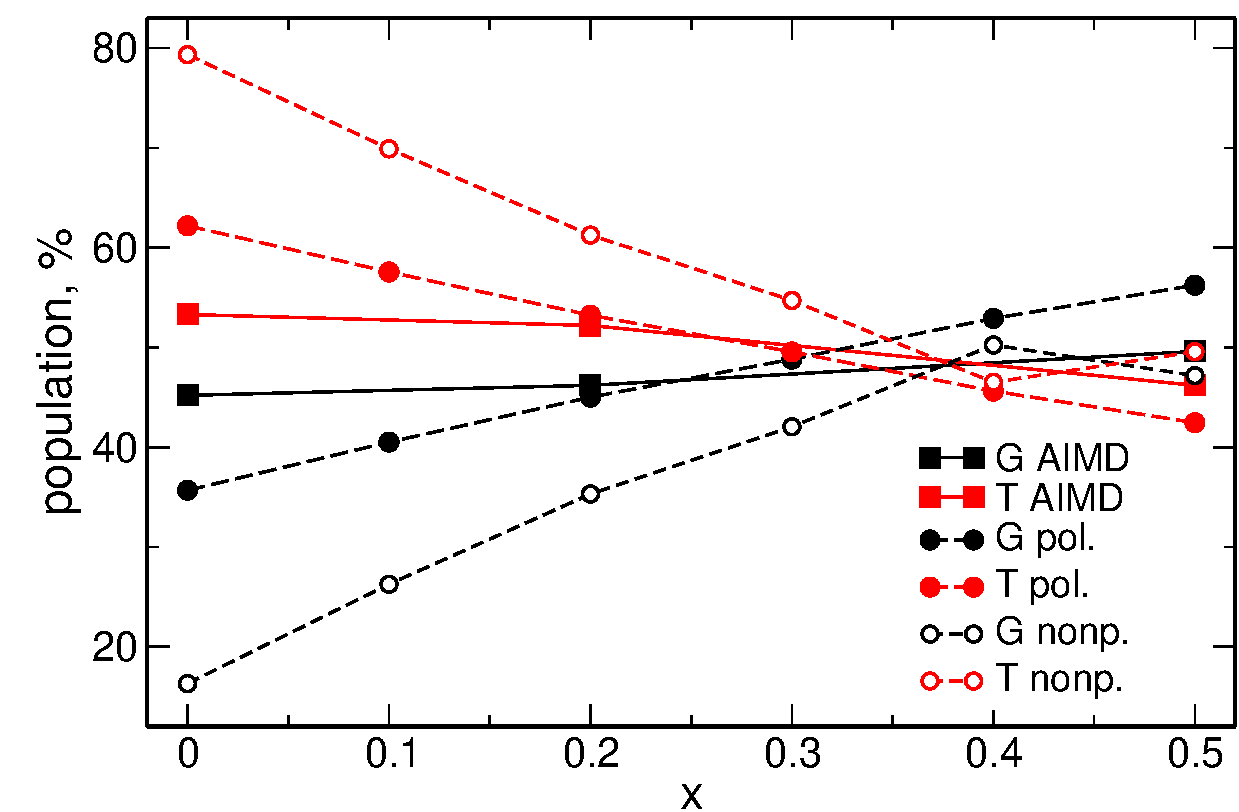
\includegraphics[width=0.45\textwidth]{img/3-structural-data-from-md-simulations/1-emim-fsi/conformers/conformer-population.png}
    \singlespacing
    \caption{Population of different FSI$^{-}$ conformers for all studied systems as a~function of the sodium salt molar fraction $x$}
    \label{fig:emim-fsi-conformer-population}
\end{figure}

\begin{figure}[H]
    \centering
    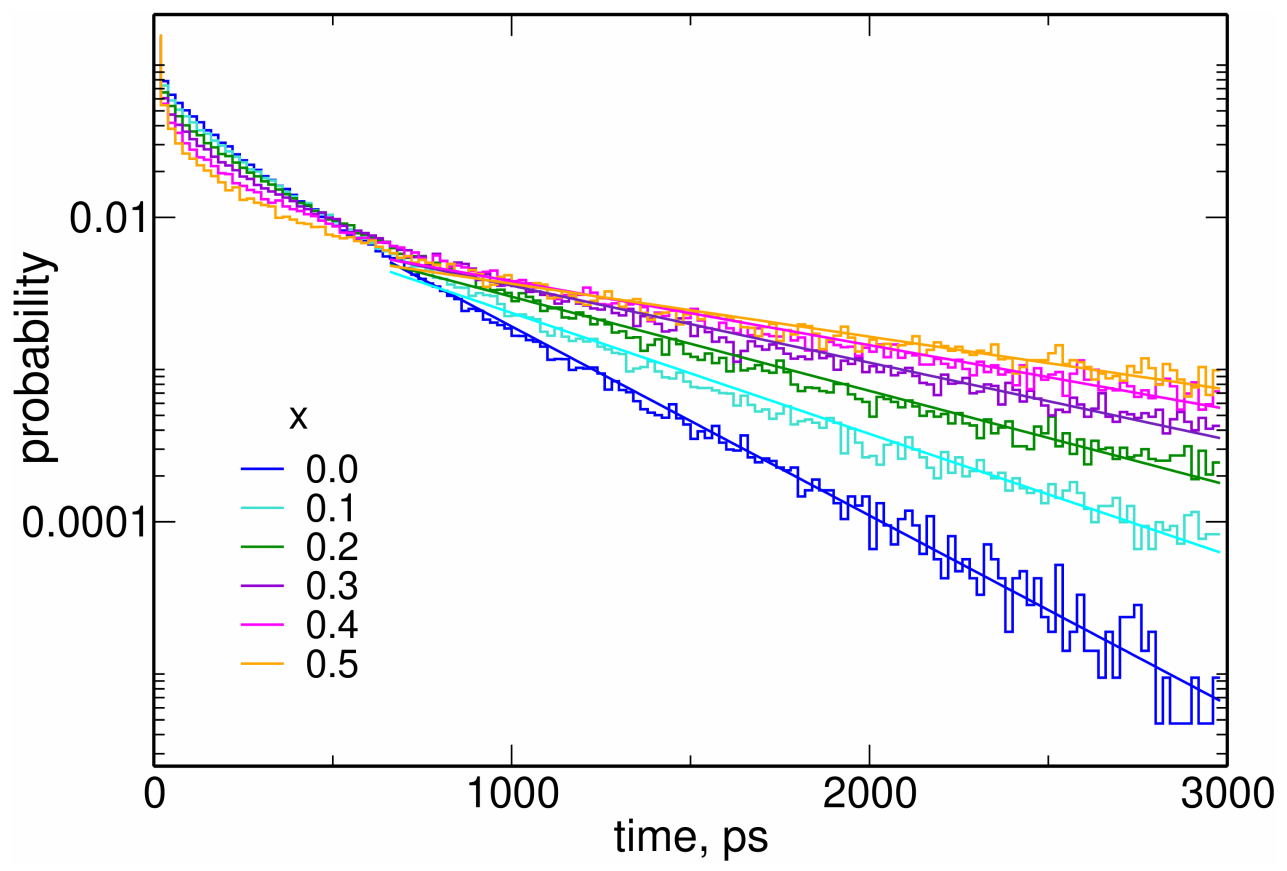
\includegraphics[width=0.45\textwidth]{img/3-structural-data-from-md-simulations/1-emim-fsi/conformers/conformer-changes-distribution.png}
    \singlespacing
    \caption{Histograms of distribution of the time between conformational changes of FSI$^{-}$ anions in DP-FF MD simulations with fitted $p = Ae^{-\frac{\tau}{t}}$ curve to the long-time parts}
    \label{fig:emim-fsi-conformer-changes-distribution}
\end{figure}

\begin{figure}[H]
    \centering
    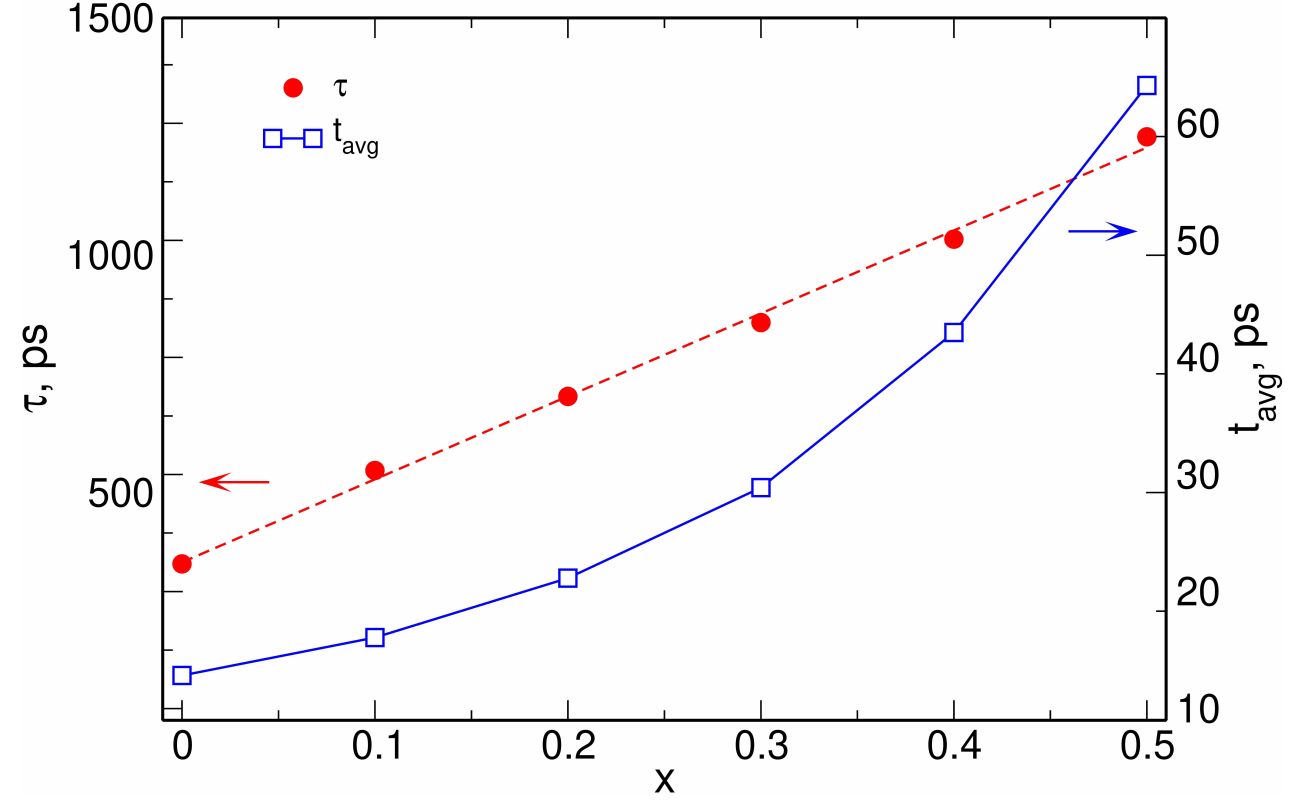
\includegraphics[width=0.45\textwidth]{img/3-structural-data-from-md-simulations/1-emim-fsi/conformers/conformer-changes-averages.png}
    \singlespacing
    \caption{Average time between conformational changes (blue) for DP-FF MD and $\tau$ parameter (defined in Figure~\ref{fig:emim-fsi-conformer-changes-distribution}) dependence on the sodium salt molar fraction $x$}
    \label{fig:emim-fsi-conformer-changes-averages}
\end{figure}

For all systems studied, the conformer population was calculated and is shown in Figure~\ref{fig:emim-fsi-conformer-population}. It was observed that, as expected, cis conformations are practically absent in every case. As suspected previously, growing Na$^{+}$ concentration changes the populations of conformers, with the reverse of the gauche / trans ratio between $x$ equal 0.3 and 0.4 for DP-FF and AIMD. For NP-FF, this ratio becomes approximately equal~1 for the most concentrated solutions. Observed changes of conformer populations with changes in NaFSI amount are smaller in AIMD. However, smaller sizes of systems studied in AIMD together with much shorter simulation times than in the FF MD give worse statistics than in the FF MD and, thus, these values have bigger error.

\begin{figure}[ht]
    \centering
    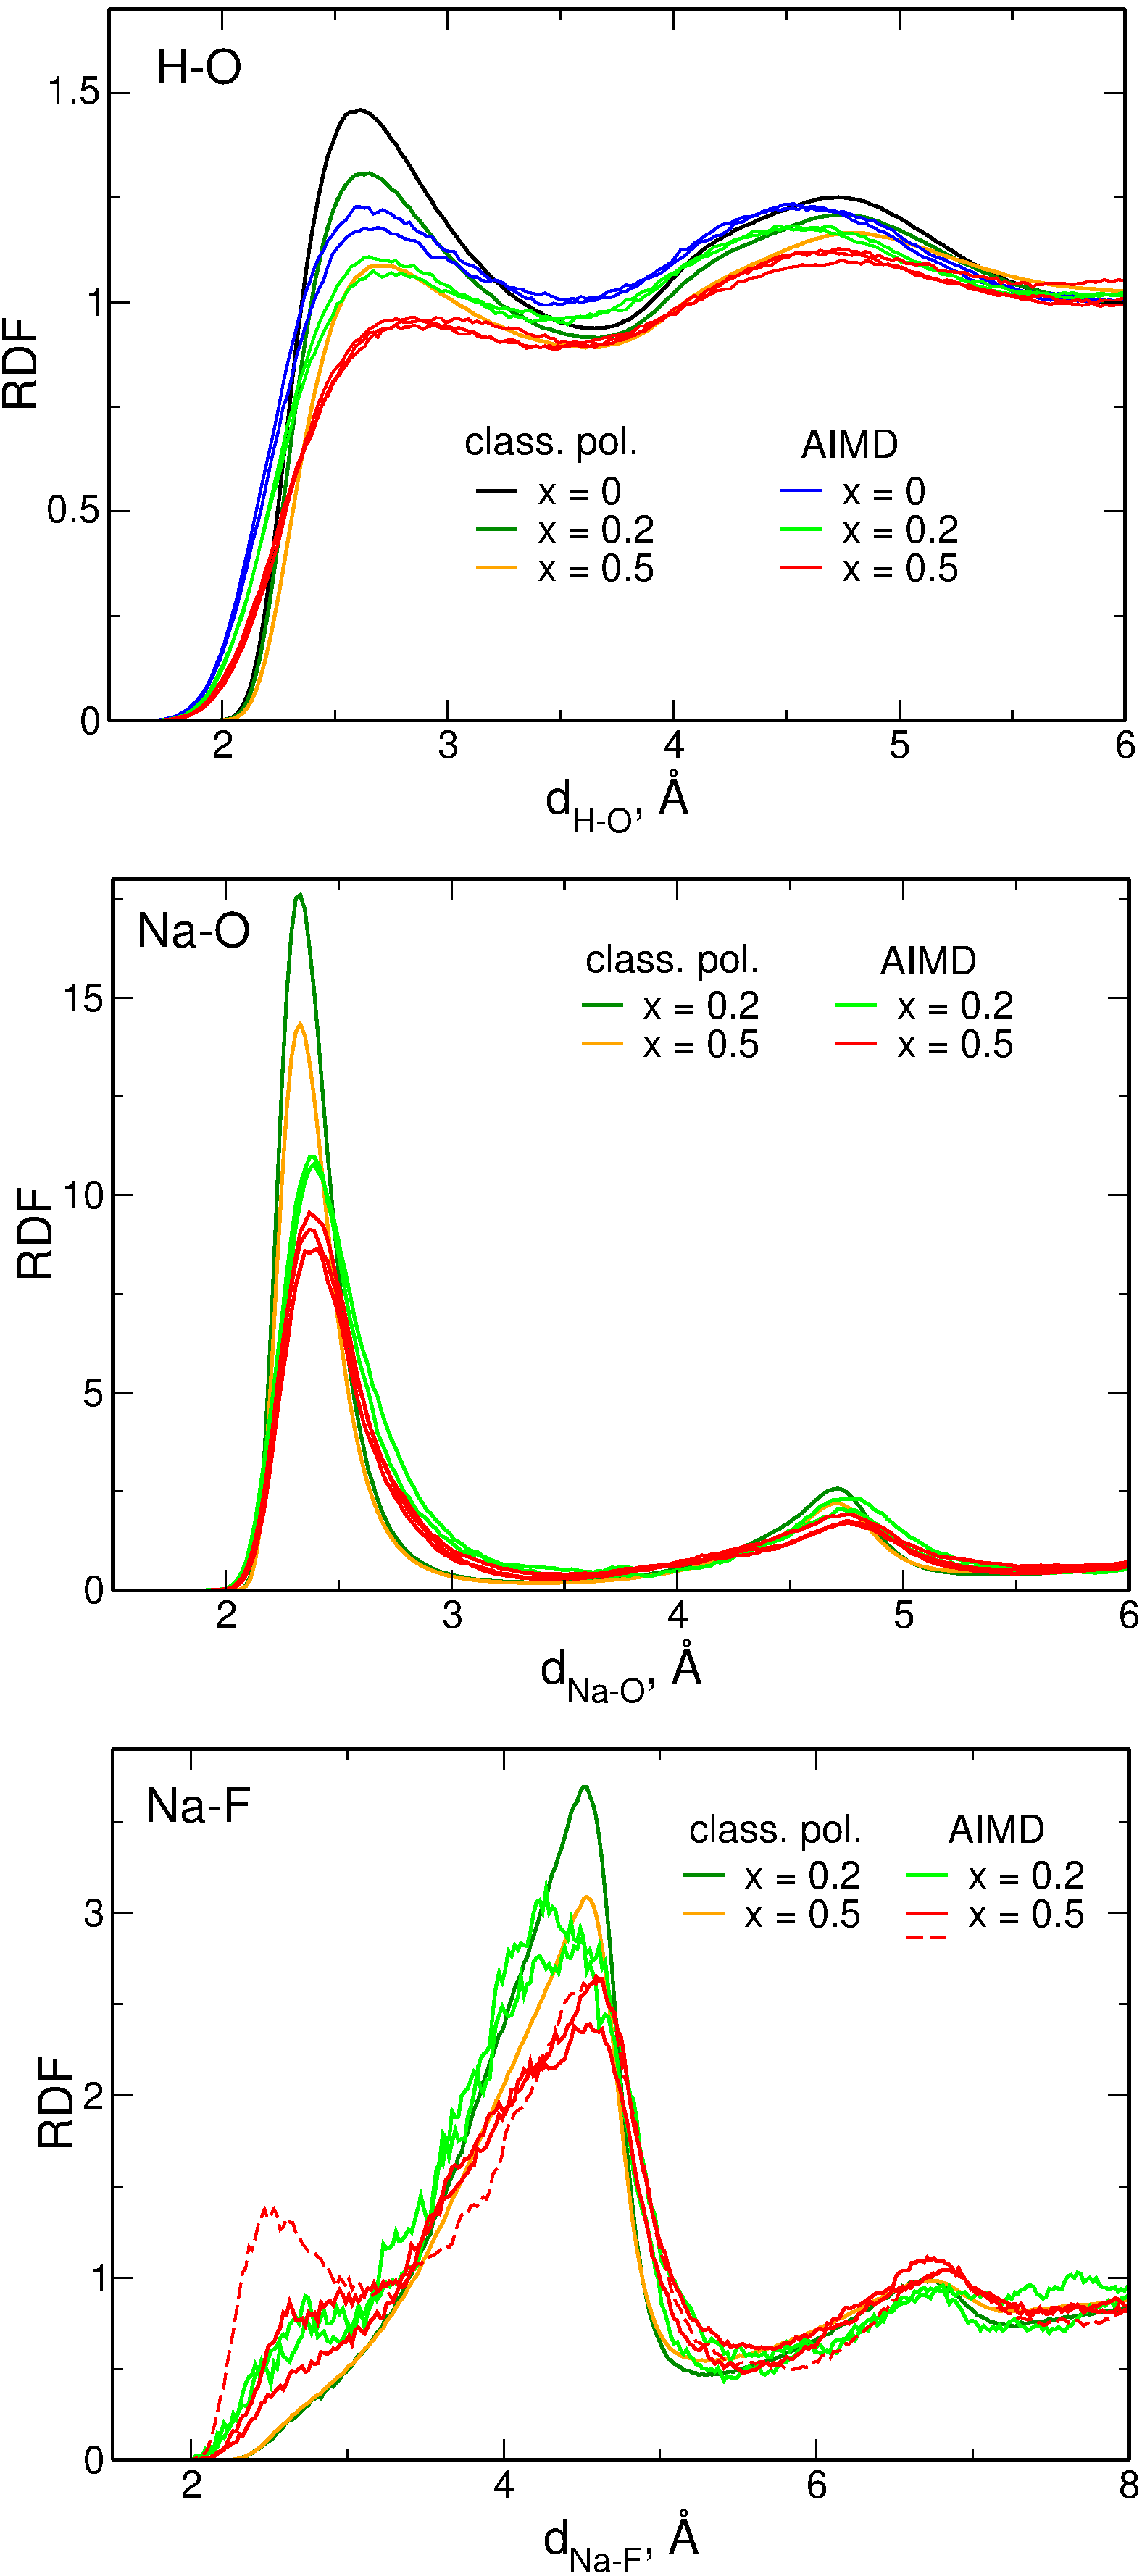
\includegraphics[width=0.45\textwidth]{img/3-structural-data-from-md-simulations/1-emim-fsi/rdf/rdf.png}
    \caption{Radial distribution functions for DP-FF MD and AIMD for systems with 0, 0.2 and 0.5 NaFSI molar fractions}
    \label{fig:emim-fsi-rdf}
\end{figure}

For systems studied by the FF MD, the dynamics of conformational changes in anions was investigated by collecting for every FSI$^{-}$ how long were the intervals between moments with changes in dihedral angles leading to changing the conformation state. Figures \ref{fig:emim-fsi-conformer-changes-distribution} and~\ref{fig:emim-fsi-conformer-changes-averages} present data obtained in DP-FF MD. It is visible, that growing sodium salt concentration slows this process with average time between conformational changes of FSI$^{-}$ anions at a~level of 13~ps for the neat liquid and about 60~ps for the most concentrated solution. The function $p = Ae^{-\frac{t}{\tau}}$ was fitted to the long-time part of the distribution in Figure~\ref{fig:emim-fsi-conformer-changes-distribution}. The $\tau$ parameter increases linearly with the salt molar fraction (Figure~\ref{fig:emim-fsi-conformer-changes-averages}) as another indication of slower conformational changes in concentrated electrolytes.

\begin{figure}[ht]
    \centering
    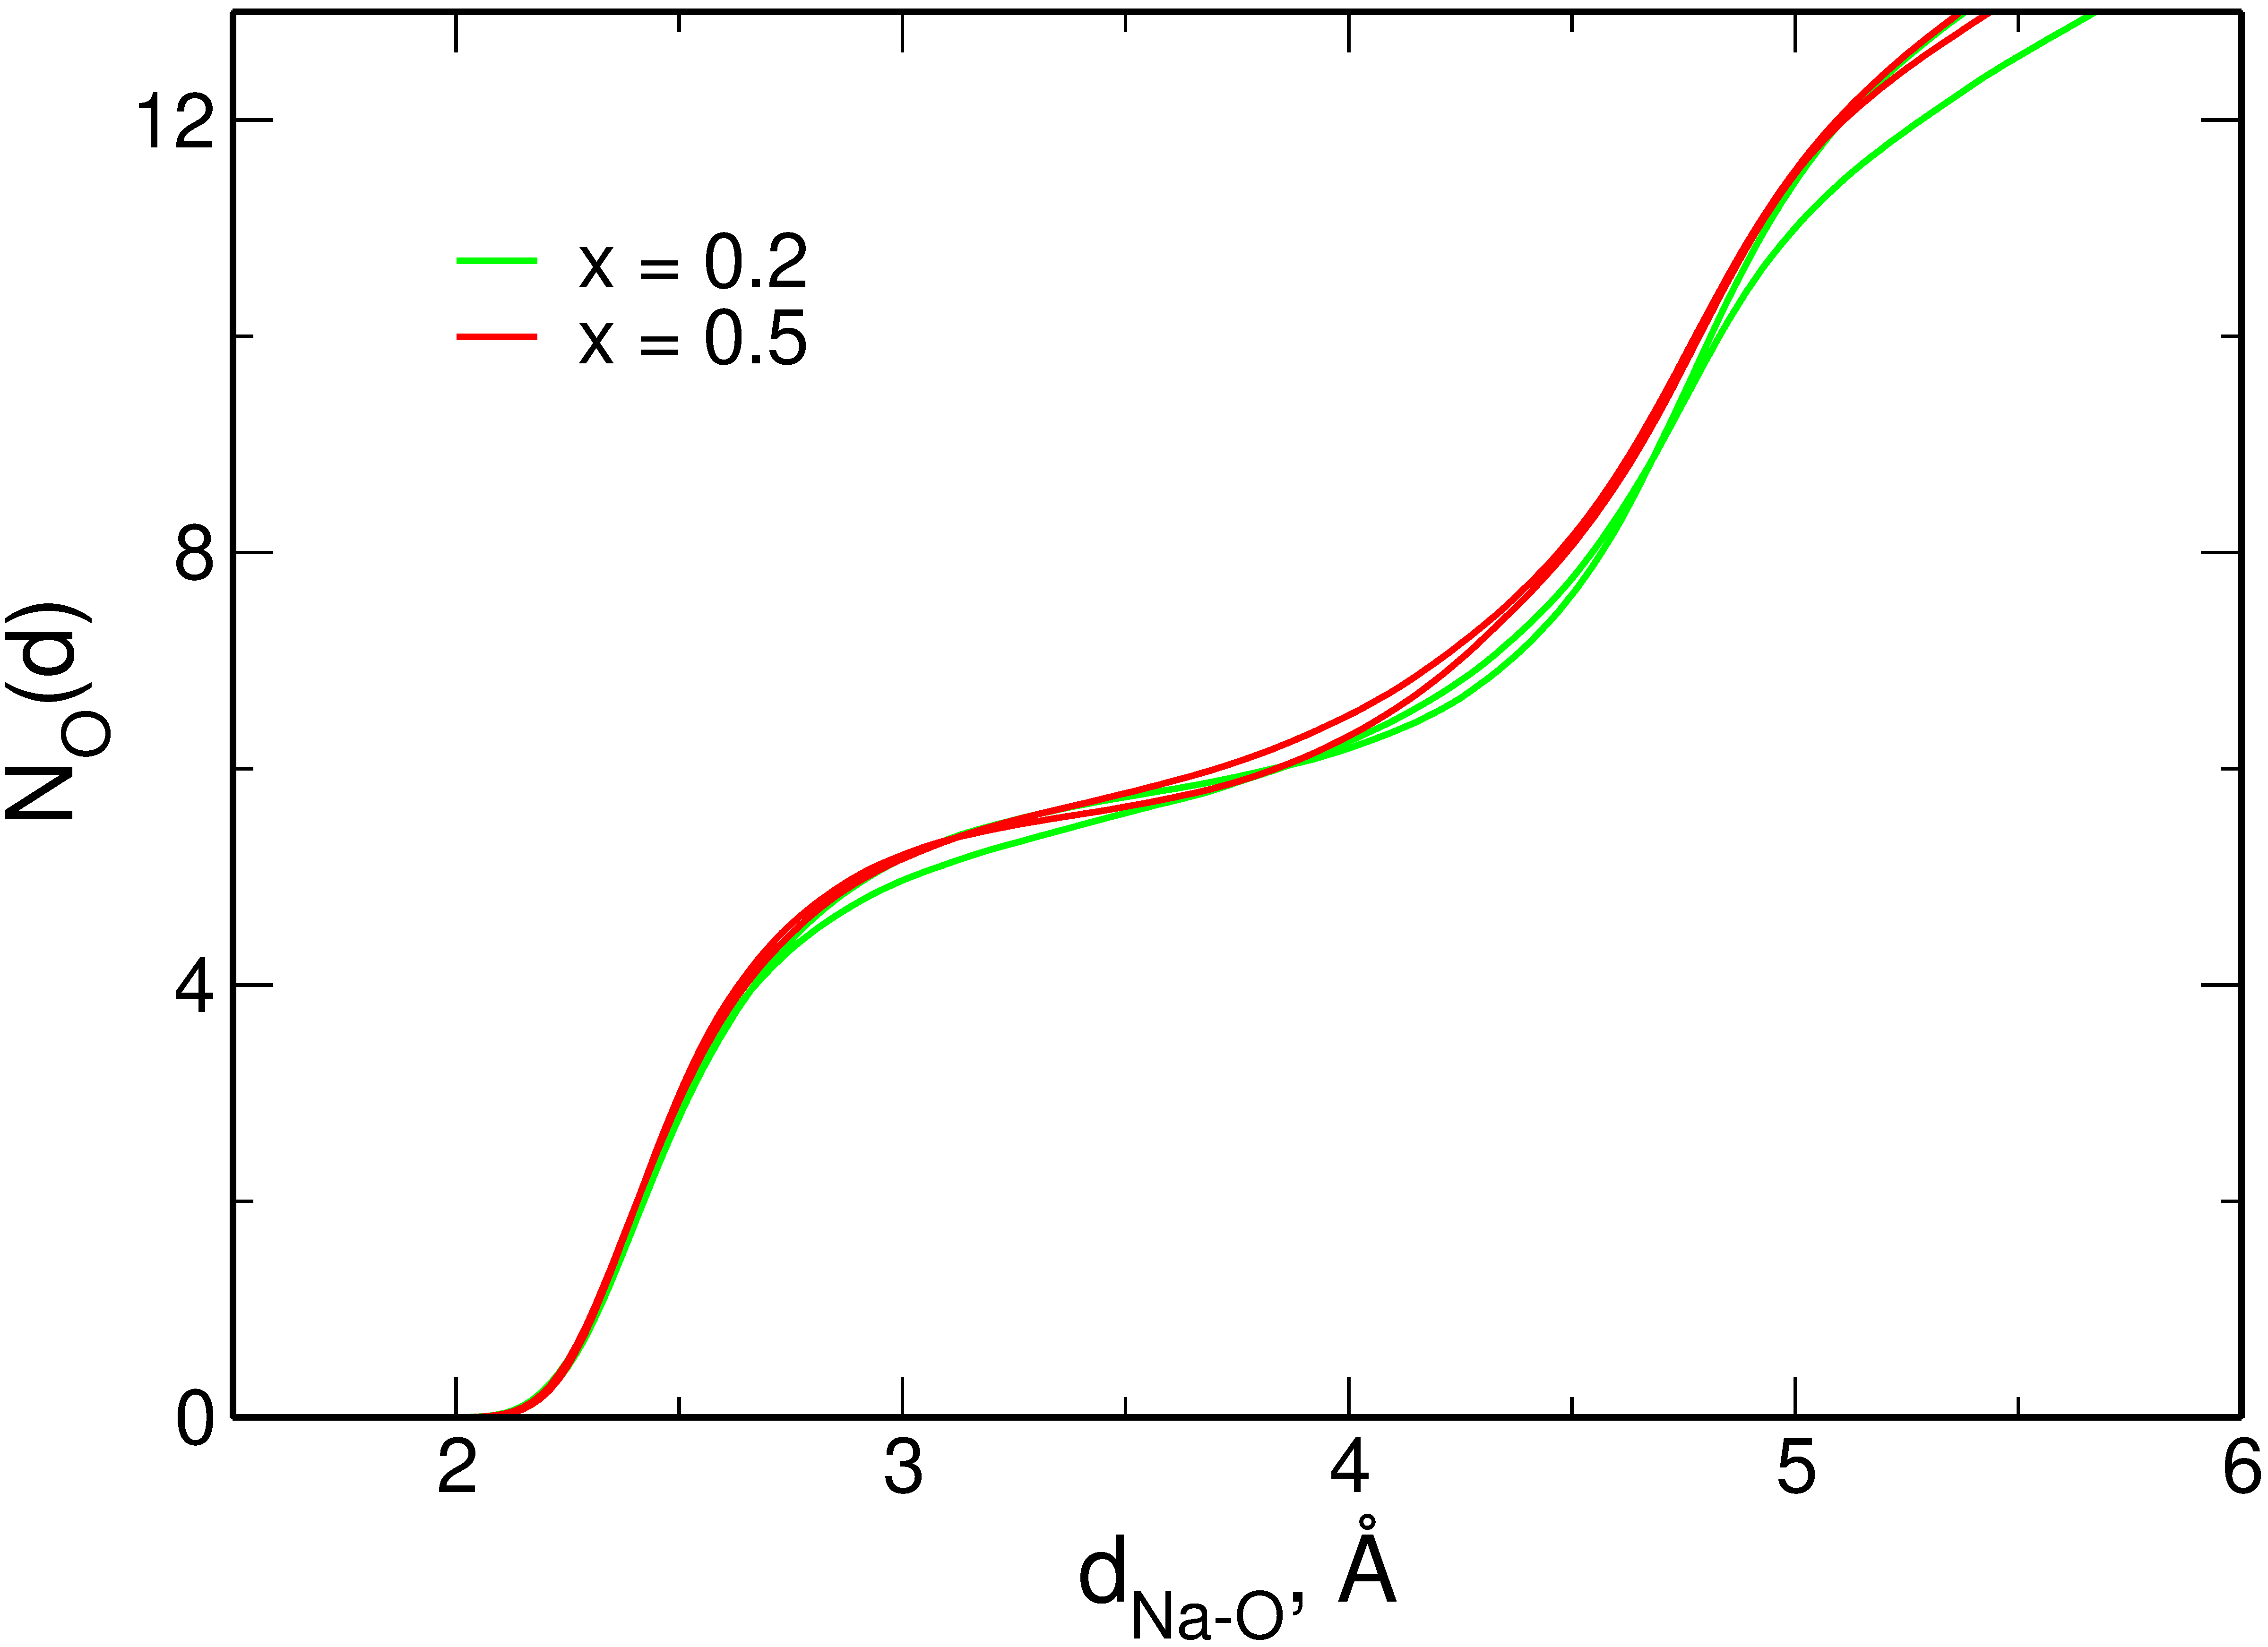
\includegraphics[width=0.4\textwidth]{img/3-structural-data-from-md-simulations/1-emim-fsi/rdf/rdf-na-o-int-aimd.png}
    \caption{Integrated Na-O RDF for AIMD simulations}
    \label{fig:emim-fsi-rdf-na-o-int-aimd}
\end{figure}

For low Na$^{+}$ concentrations, the trans conformers are more abundant, but interactions with Na$^{+}$ stabilize the gauche conformation of the FSI$^{-}$ anion in concentrated salt solutions. An analogous effect of the stabilization of gauche conformer was experimentally observed from Raman spectra of EMIM-FSI liquid with LiFSI salt~\cite{li-emim-fsi-solvation}.

\begin{figure}[ht]
    \centering
    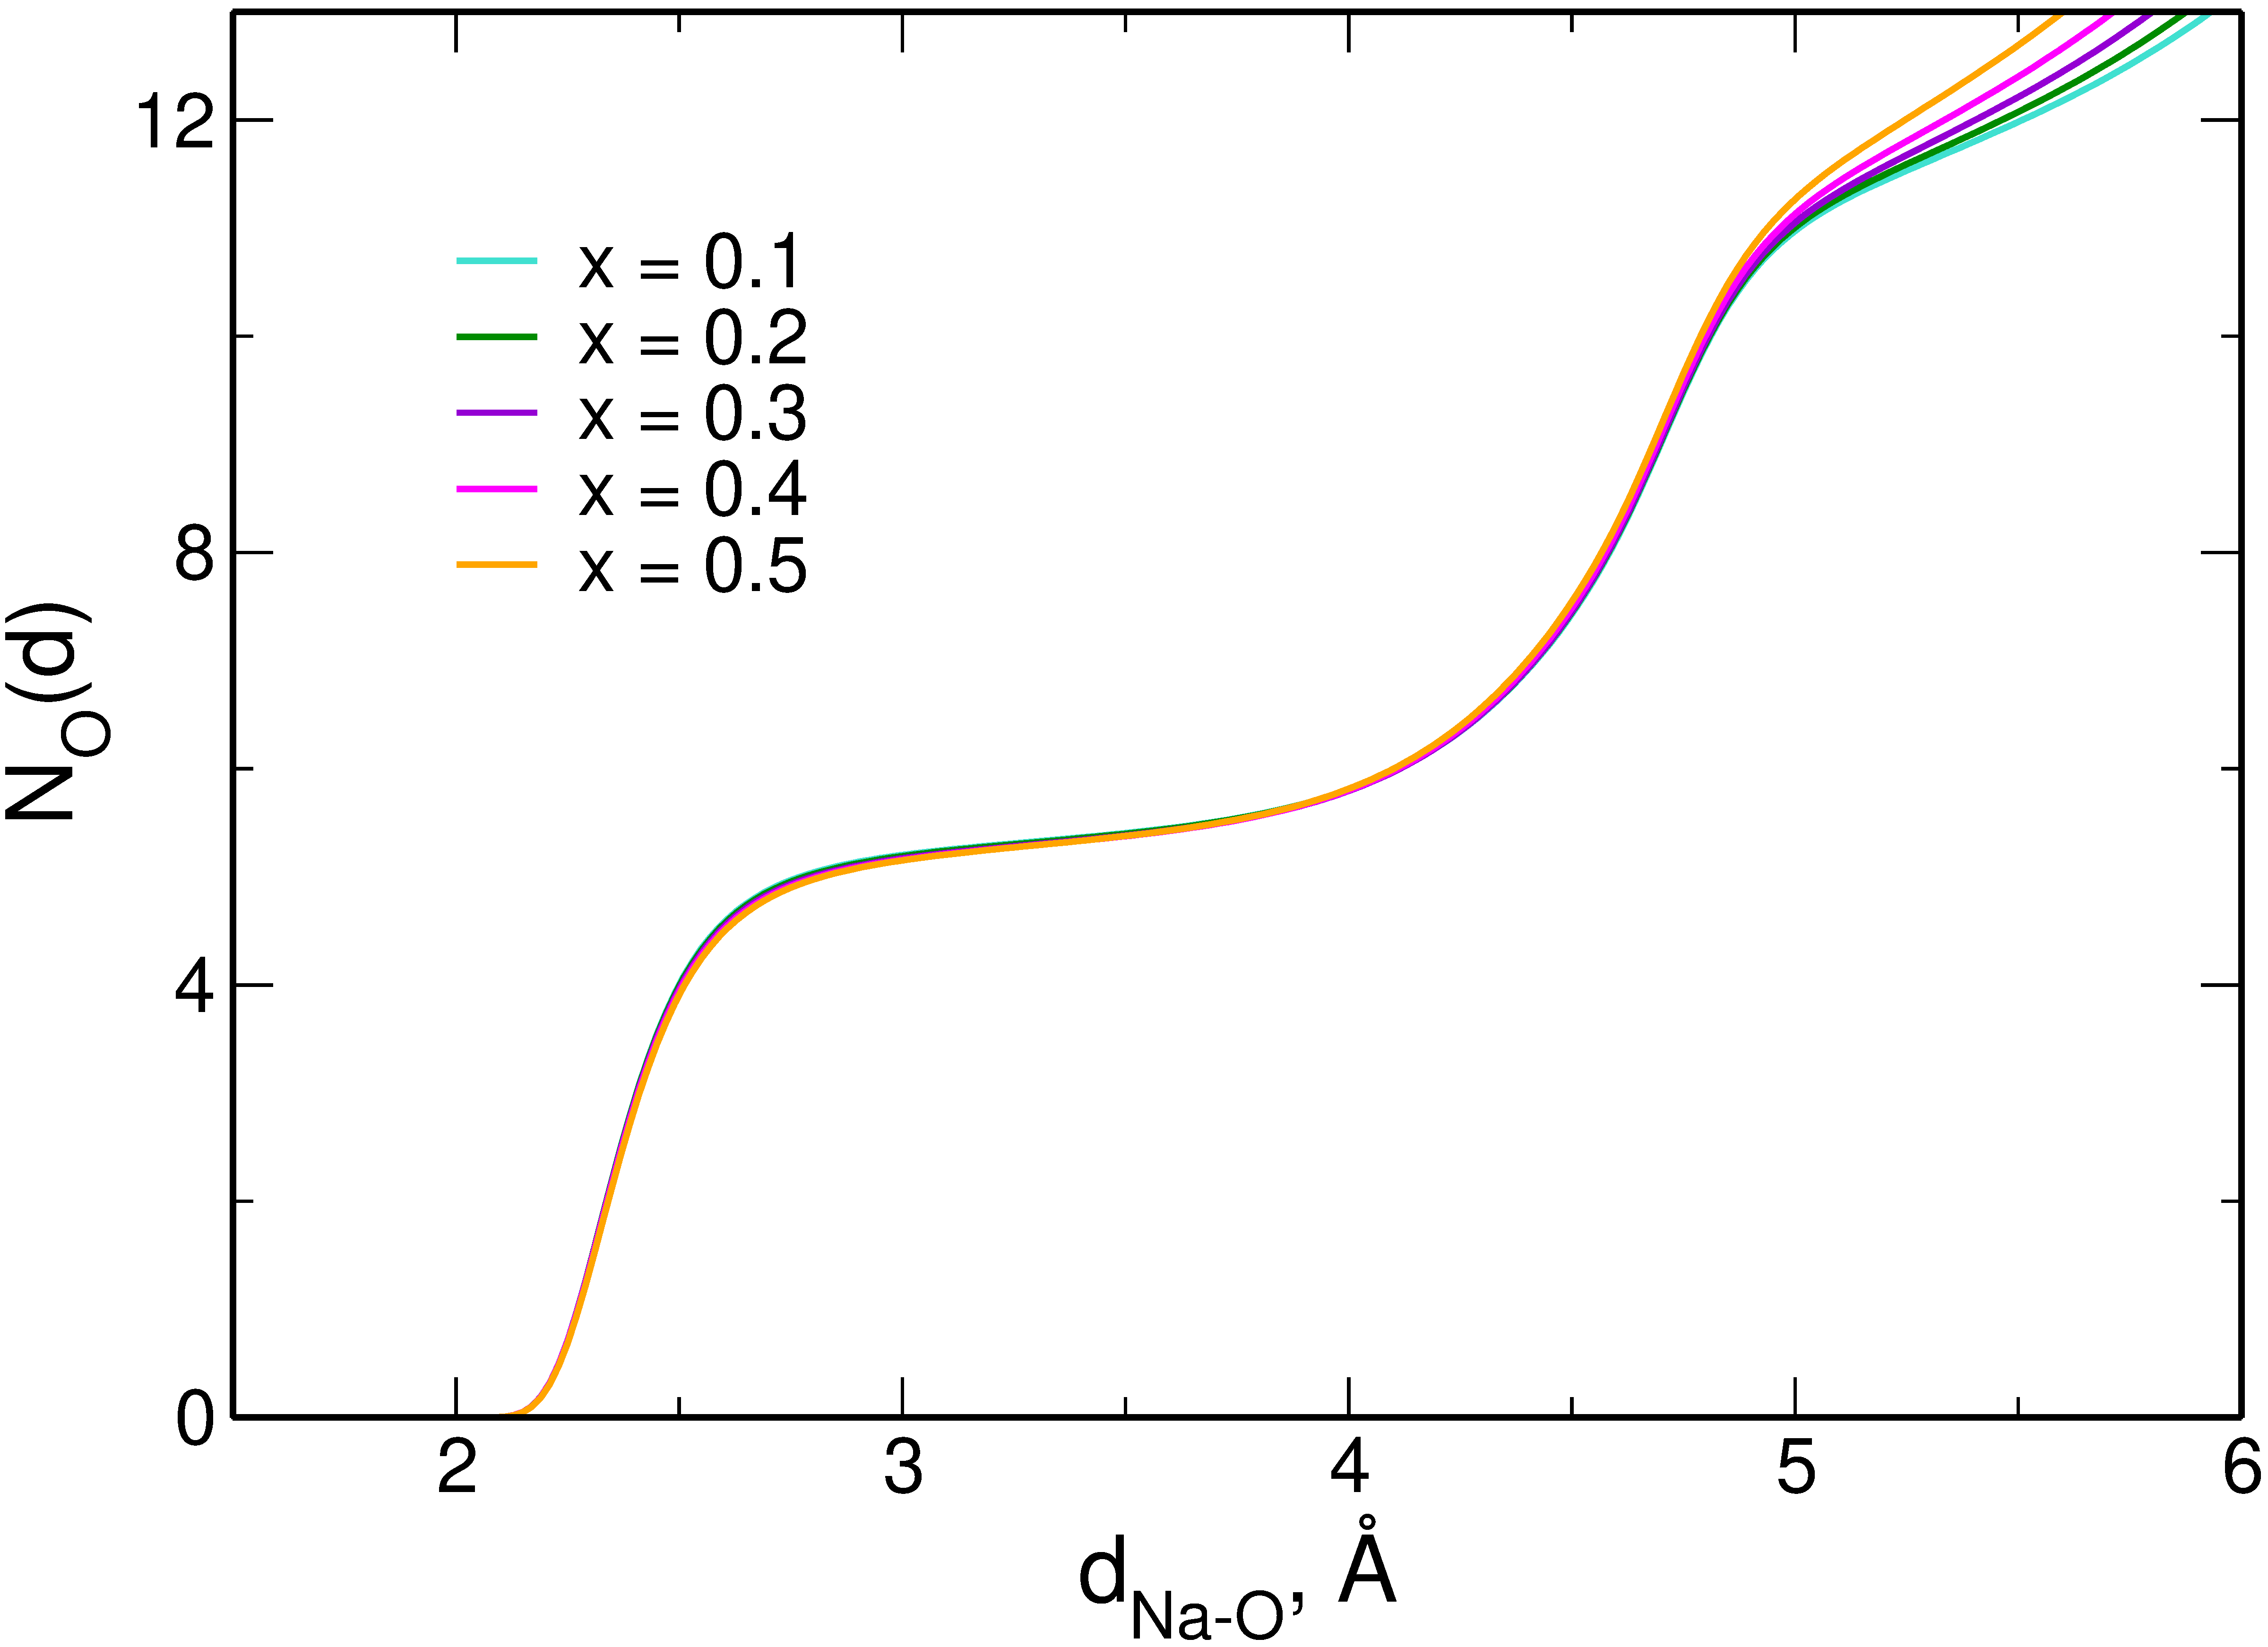
\includegraphics[width=0.4\textwidth]{img/3-structural-data-from-md-simulations/1-emim-fsi/rdf/rdf-na-o-int-dpff.png}
    \caption{Integrated Na-O RDF for DP-FF simulations}
    \label{fig:emim-fsi-rdf-na-o-int-dpff}
\end{figure}

Figure~\ref{fig:emim-fsi-rdf} shows the radial distribution functions (RDFs) for DP-FF MD and AIMD for systems with concentrations which were used in AIMD for H-O, Na-F and Na-O distances. In general, positions of maxima agree between these two methods, however, the peaks observed in AIMD are lower than those observed in DP-FF MD.

In the H-O RDF, the first maximum is located at 2.6-2.7~{\AA}. For both simulation methods, its height decreases with growing concentration of the sodium salt and shifts to higher distances. It is probably related to the weakening of the hydrogen bonds between ions of the IL with the addition of sodium salt.

\begin{figure}[H]
    \centering
    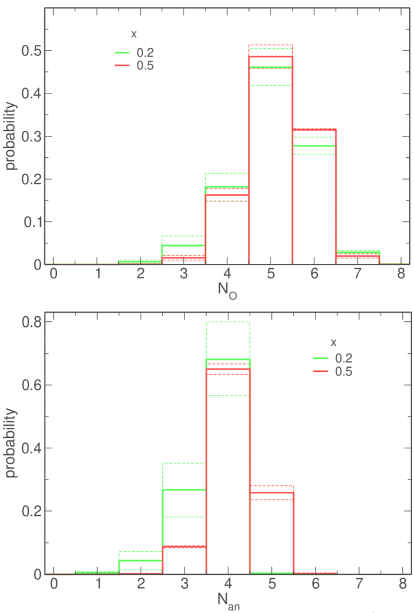
\includegraphics[width=0.38\textwidth]{img/3-structural-data-from-md-simulations/1-emim-fsi/rdf/stat-aimd.png}
    \singlespacing
    \caption{Histograms of the number of O atoms (N$_O$) coordinating sodium cations (upper) and number of different FSI$^{-}$ anions (N$_{an}$) in sodium solvation shell for AIMD simulations (lower). Solid lines are average values over all studied systems at a~given concentration $x$ (shown in broken lines)}
    \label{fig:emim-fsi-rdf-stat-aimd}
\end{figure}

\begin{figure}[H]
    \centering
    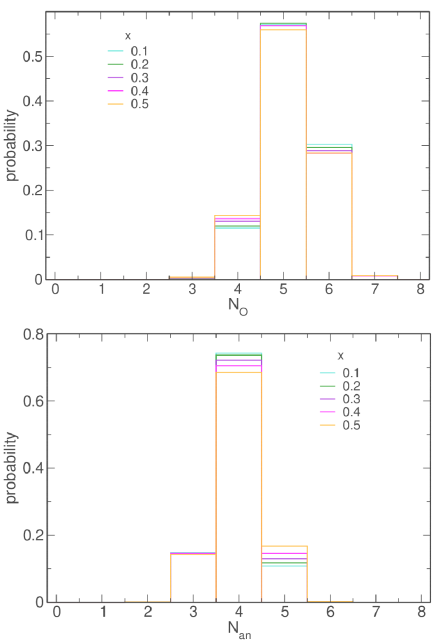
\includegraphics[width=0.38\textwidth]{img/3-structural-data-from-md-simulations/1-emim-fsi/rdf/stat-dpff.png}
    \singlespacing
    \caption{Histograms of the number of O atoms (N$_O$) coordinating sodium cations (upper) and number of different FSI$^{-}$ anions (N$_{an}$) in sodium solvation shell for DP-FF simulations (lower)}
    \label{fig:emim-fsi-rdf-stat-dpff}
\end{figure}

Comparison of positions and heights of the first maxima in Na-O and Na-F RDFs clearly shows that Na$^{+}$ cations are mostly coordinated by oxygen atoms from FSI$^{-}$ anions. It is worth noting that one of the systems with $x = 0.5$ studied in AIMD has the Na-F RDF (marked with the dashed line) differing from the others. This difference will be addressed in the further text. The position of the first maximum of Na-O RDF in the DP-FF MD is at distance smaller than in AIMD. The integrated RDFs (running coordination numbers) presented in Figures~\ref{fig:emim-fsi-rdf-na-o-int-aimd} and~\ref{fig:emim-fsi-rdf-na-o-int-dpff} show that the average number of~O atoms in the first solvation shell of sodium cation is equal 5.6 for AIMD and 5.4 for DP-FF simulations.

\begin{figure}[ht]
    \centering
    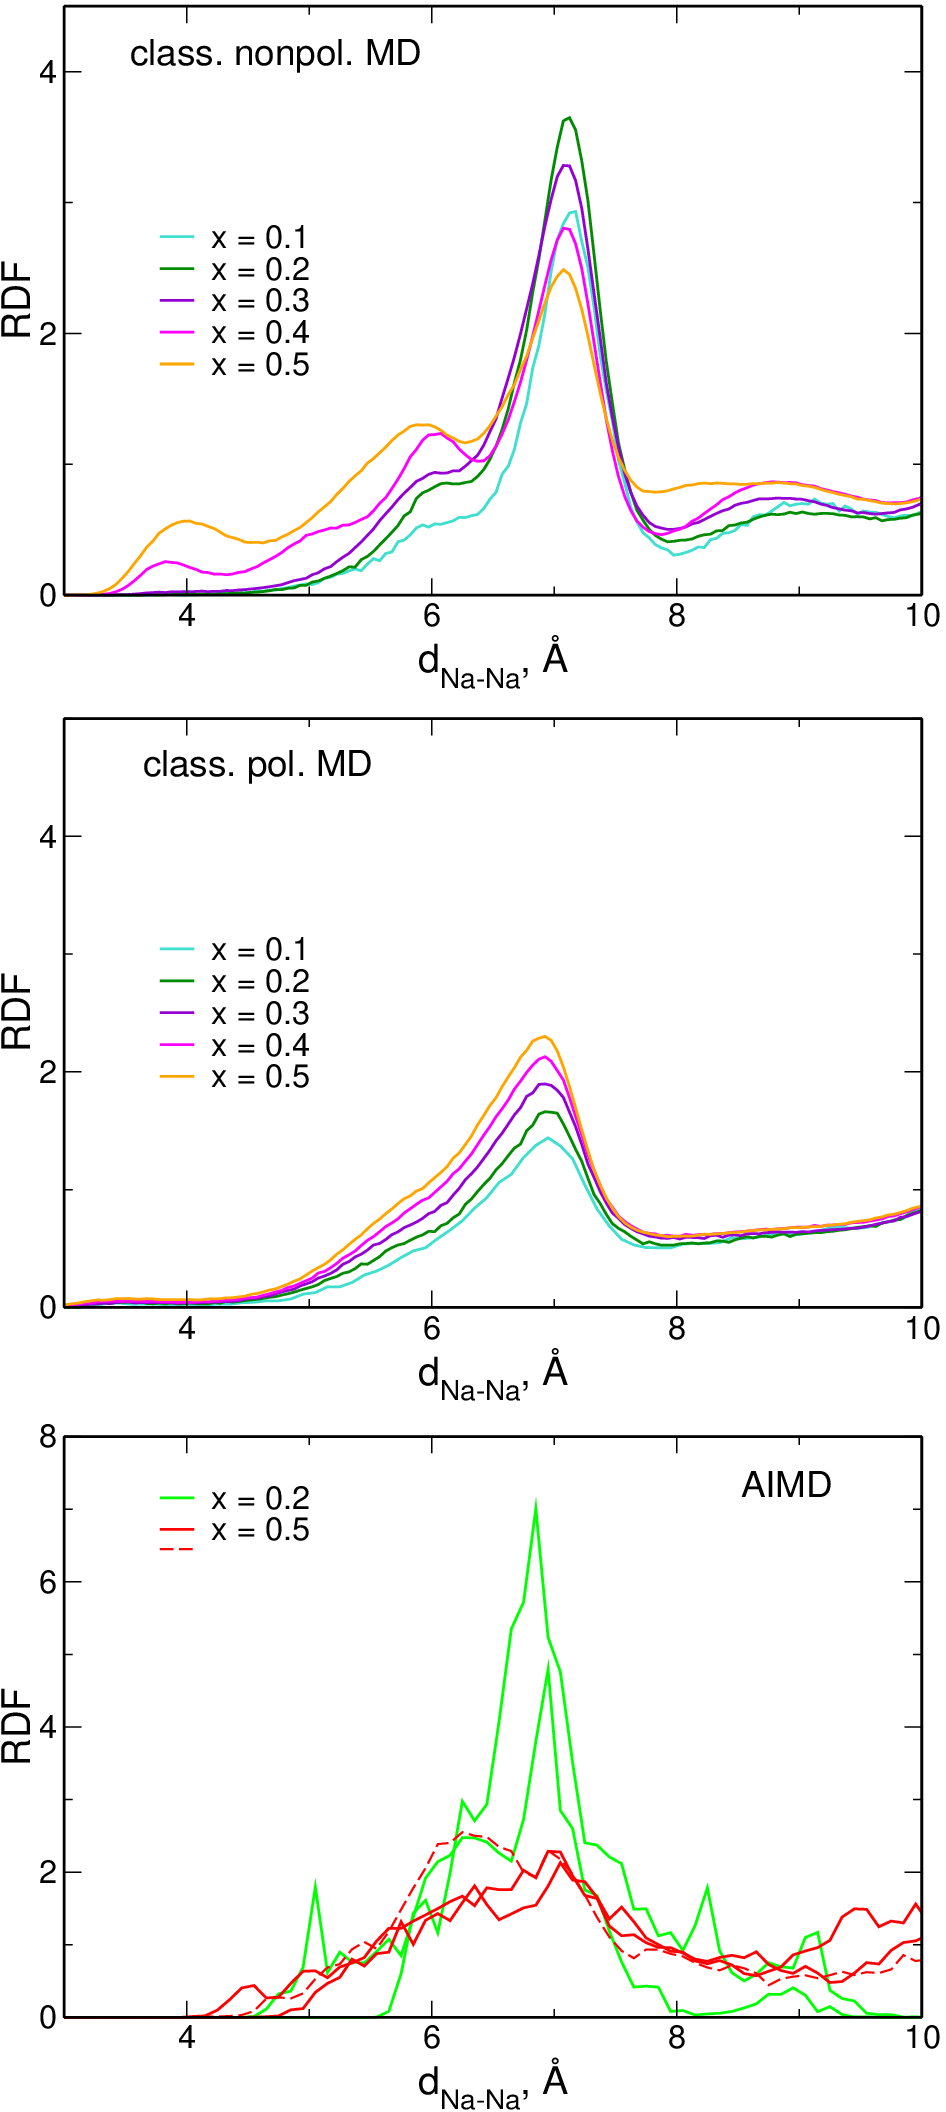
\includegraphics[width=0.45\textwidth]{img/3-structural-data-from-md-simulations/1-emim-fsi/rdf/rdf-na-na.png}
    \caption{Radial distribution functions for Na-Na}
    \label{fig:emim-fsi-rdf-na-na}
\end{figure}

Figures~\ref{fig:emim-fsi-rdf-stat-aimd} and~\ref{fig:emim-fsi-rdf-stat-dpff} show statistics of sodium coordination both in AIMD and DP-FF MD simulations. In both of them above 50\% of Na$^{+}$ cations are coordinated by five oxygen atoms and about 30\% by six. Above 60\% of complexes are in the form [Na(FSI)$_4$]$^{3-}$, what shows that in most of them three anions are coordinated in monodentate manner and one in bidentate. Complexes with coordination number equal 6~may have two anions with monodentate coordination and two with bidentate. In AIMD results, for the system with $x = 0.5$, about 25\% of sodium cations are in the form [Na(FSI)$_5$]$^{4-}$ without significant increase in the average coordination number, thus with growing salt concentration, monodentate coordination becomes more preferred. From these plots also smaller changes in coordination patterns with changing NaFSI concentration in DP-FF MD compared to AIMD are observed. However, this difference could be an effect od worse statistics of AIMD results (smaller systems, shorter simulation times).

\begin{figure}[ht]
    \centering
    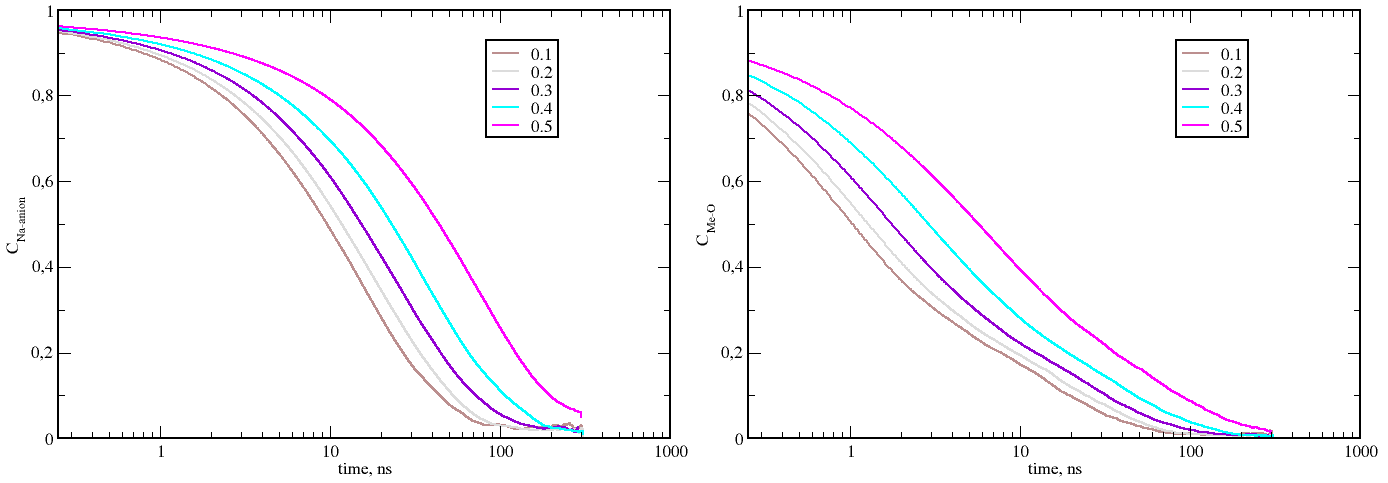
\includegraphics[width=0.9\textwidth]{img/3-structural-data-from-md-simulations/1-emim-fsi/autocorrelation/residence.png}
    \caption{Residence time autocorrelation functions for DP-FF for Na$^{+}$ coordination by whole anions (left) and individual O~atoms (right)}
    \label{fig:emim-fsi-residence}
\end{figure}

Figure~\ref{fig:emim-fsi-rdf-na-na} shows RDFs for Na-Na pairs. Due to poor statistics, the AIMD results are noisy. In FF approaches wide maximum at about 7~{\AA} is observed and for higher concentrations in NP-FF two weaker maxima appear at lower distances; thus, some kind of weak ordering of metal ions may occur in concentrated solutions.

In Figure~\ref{fig:emim-fsi-rdf-na-na} dashed line marks the $x = 0.5$ system, which previously exhibited a different behavior from other $x = 0.5$ systems in Na-F RDF (Figure~\ref{fig:emim-fsi-rdf}). Also in the case of the Na-Na RDF, its maximum is shifted toward lower values than those of replicas with this salt concentration. It suggests that this would give different results in other properties, such as IR spectra discussed in Section~\ref{section:emim-fsi-ir}. In addition, is may be expected that for sufficiently long times of simulation these differences could vanish.

Figure~\ref{fig:emim-fsi-residence} presents residence time autocorrelation functions (AFs) calculated for DP-FF MD simulations, both for coordination by whole anions and for individual O~atoms. In both plots, it is visible that the higher the salt concentration, the slower the decay of $C(t)$. For given concentration, AF for individual~O atoms decreases faster than for the whole anion. From these results, it could be deduced that for concentrated solutions, exchanges in the coordination shells are slower, and that it takes a~longer time for exchange of the anion than of the single O~atom. It is related to the fact that exchange of the anion requires breaking all coordination bonds to the cation.

\cleardoublepage